% -*-LaTex-*-

%-----------------------------------------------------------------------------
%   Copyright 2016 Florian Schumacher (Ruhr-Universitaet Bochum, Germany)
%
%   This file is part of the ASKI manual as a LaTeX document with main file
%   manual.tex
%
%   Permission is granted to copy, distribute and/or modify this document
%   under the terms of the GNU Free Documentation License, Version 1.3
%   or any later version published by the Free Software Foundation;
%   with no Invariant Sections, no Front-Cover Texts, and no Back-Cover Texts.
%   A copy of the license is included in the section entitled ``GNU
%   Free Documentation License''. 
%-----------------------------------------------------------------------------
%
In general, in this chapter we provide only basic information. For more detail on 
specific steps or objects, we always refer to the respective sections below in this document.
%
%++++++++++++++++++++++++++++++++++++++++++++++++++++++++++
\section{Installing \ASKI} \label{basic_steps,sec:install_ASKI}
%++++++++++++++++++++++++++++++++++++++++++++++++++++++++++
%
\begin{itemize}
\item Download main package \lcode{ASKI_1.1.tar.gz} from \url{http://www.rub.de/aski}
\item Unpack tar ball (containing the directory \lcode{ASKI_1.1/}) somewhere
\item Follow the directions in file \lcode{ASKI_1.1/README}
\end{itemize}
%
%++++++++++++++++++++++++++++++++++++++++++++++++++++++++++
\section{Create Main Parameter File} \label{basic_steps,sec:main_parfile}
%++++++++++++++++++++++++++++++++++++++++++++++++++++++++++
%
The simplest way to create a specific main parameter file for your operation is to modify / adjust 
a copy of the template file \lcode{template/main_parfile_template}. 

Refer to the commented documentation in \lcode{main_parfile_template} or 
to sections~\myref{files,sec:parfiles} and~\myref{files,sec:main_parfile}.
%
%++++++++++++++++++++++++++++++++++++++++++++++++++++++++++
\section{Iteration Step Parameter Files} \label{basic_steps,sec:iter_parfile}
%++++++++++++++++++++++++++++++++++++++++++++++++++++++++++
%
Having created a directory environment for your operation, as described in section~\myref{basic_steps,sec:create_dir},
there should automatically have been created template
parameter files in each directory of an iteration step, having filenames as defined by
parameter \lcode{PARFILE_ITERATION_STEP} in the main parameter file.

Refer to the commented documentation in those template files or 
to sections~\myref{files,sec:parfiles} and~\myref{files,sec:iter_parfile}.
%
%++++++++++++++++++++++++++++++++++++++++++++++++++++++++++
\section{Create Directory Environment} \label{basic_steps,sec:create_dir}
%++++++++++++++++++++++++++++++++++++++++++++++++++++++++++
%
Call python script \lcode{create_ASKI_dir.py}
\begin{lstlisting}
USAGE: please give 2 arguments:
[1] main parmeter file of inversion
[2] number of iteration steps

EXAMPLE:
create_ASKI_dir.py ./main_parfile_Aegean1 10
\end{lstlisting}
Put your main parameter file (see~\myref{basic_steps,sec:main_parfile}) as the first, and the expected 
number of iteration steps as the second argument. \\
You can always \emph{recall this script at any later time} with a larger number of iteration steps. 
All existing directories \emph{will not be affected}, only additional non-existing objects will be 
created. Recalling this script with a smaller number of steps will not delete anything.
%
%++++++++++++++++++++++++++++++++++++++++++++++++++++++++++
\section{Data in \ASKI} \label{basic_steps,sec:data_general}
%++++++++++++++++++++++++++++++++++++++++++++++++++++++++++
%
One certain data sample in \ASKI{} is characterized by a seismic \emph{source}, a \emph{component} 
of a seismic \emph{station} (receiver), and a \emph{frequency}, as well as if it is \emph{real} or \emph{imaginary} part 
of the complex spectral values. It has the value of displacement of the ground in the unit of meters.
%
%----------------------------------------------------------
\subsection*{Events and Stations}
%----------------------------------------------------------
%
The events file (\myref{files,sec:event_list}) and stations file (\myref{files,sec:station_list}) constitute a
collection of \emph{all} events (stations) which will be involved \emph{in any way} in your \ASKI{} operation.\\
All programs/scripts will refer to a specific event (station) by its event-ID (station-name).
%
%----------------------------------------------------------
\subsection*{Station Components}
%----------------------------------------------------------
%
All programs/scripts will refer to a specific station component by the following abbreviatory names.\\
Dependent on the coordinate system in which the stations are defined (Cartesian or spherical, which is 
defined by the first line of the station list file), the supported names of station components may have a 
different meaning:
\subsubsection{Cartesian stations}
\begin{itemize}
\item[] \lcode{CX}: Cartesian \lcode{X}-coordinate (first Cartesian coordinate)
\item[] \lcode{CY}: Cartesian \lcode{Y}-coordinate (second Cartesian coordinate)
\item[] \lcode{CZ}: Cartesian \lcode{Z}-coordinate (third Cartesian coordinate)
\item[] \lcode{N}: same as \lcode{-CX}
\item[] \lcode{S}: same as \lcode{CX}
\item[] \lcode{E}: same as \lcode{CY}
\item[] \lcode{W}: same as \lcode{-CY}
\item[] \lcode{UP}: same as \lcode{CZ}
\item[] \lcode{DOWN}: same as \lcode{-CZ}
\end{itemize}
\subsubsection{Spherical stations}
\begin{itemize}
\item[] \lcode{CX}: Cartesian \lcode{X}-coordinate with \lcode{X}-axis through equator and $0^\circ$-meridian
\item[] \lcode{CY}: Cartesian \lcode{Y}-coordinate with \lcode{Y}-axis through equator and $90^\circ$E-meridian
\item[] \lcode{CZ}: Cartesian \lcode{Z}-coordinate with \lcode{Z}-axis through north pole
\item[] \lcode{N}: local north
\item[] \lcode{S}: local south
\item[] \lcode{E}: local east
\item[] \lcode{W}: local west
\item[] \lcode{UP}: local up
\item[] \lcode{DOWN}: local down
\end{itemize}
%
%----------------------------------------------------------
\subsection*{Frequency Discretization}
%----------------------------------------------------------
%
In \ASKI{}, frequencies are given by a frequency step $\Delta f$[Hz] and by a set of integer valued 
frequency indices.

For specific frequency index $k\in\mathbb{N}$, the corresponding real-valued frequency $f_k$ [Hz] computes as
$f_k \,=\, k \,\cdot\, \Delta f$.
E.g.\ $\Delta f \,=\, 10$ Hz and frequency indices $k \,=\, 2,\; 3,\; 5,\; 7,\; 10$ define the set of 
discrete frequencies $f_k \,=\, 20.0,\; 30.0,\; 50.0,\; 70.0,\; 100.0$ [Hz].

Some forward methods (at the moment only Gemini) implicitely use \emph{complex} frequencies, which are related
to the above definition of real-valued frequencies $f_k \,=\, k \,\cdot\, \Delta f$.
Gemini, e.g., adds to these real-valued frequencies a constant imaginary part $\sigma = -5\Delta f/2\pi$,
thus implicitely using the complex frequencies $f_k \,=\, k \cdot \Delta f \,+\,i\cdot \sigma$,
where $i$ is the imaginary unit.
%
%++++++++++++++++++++++++++++++++++++++++++++++++++++++++++
\section{Prepare Measured Data} \label{basic_steps,sec:measured_data}
%++++++++++++++++++++++++++++++++++++++++++++++++++++++++++
%
For measured data given in some basic data formats like Seismic Unix and time-series given as textfiles per trace,
the executable \lcode{createMeasuredData} \myaref{programs_scripts,sec:bin_prog,sec:create_measured_data} 
converts the time-domain data to the special frequency-domain
form required by \ASKI{}. Executing \lcode{createMeasuredData} (without arguments), will print a short help message how to use it.

Otherwise you might well prepare measured data files on your own as required by \ASKI{}, see sections~\myref{basic_steps,sec:data_general} 
and~\myref{files,sec:measured_data}. 
%
%++++++++++++++++++++++++++++++++++++++++++++++++++++++++++
\section{Prepare Frequency-Domain Filters} \label{basic_steps,sec:filters}
%++++++++++++++++++++++++++++++++++++++++++++++++++++++++++
%
In \ASKI{}, synthetic wavefields (for synthetic data and sensitivity kernels) are preferred to 
be modelled as impulse responses, i.e.\ w.r.t.\ an impulsive Dirac source-time-function, and filtered afterwards
in the frequency domain (by multiplication of wavefield spectra and spectral filter) before being compared to 
measured data. Therefore, \ASKI{} uses spectral filters,
independently associated with each seismic source and each station component. This way, independent 
source-time-functions for each event, as well as independent instrument responses for each station component
can be modelled. Whether or not to use event-associated filters or station-associated filters at all, is 
controlled in the main parameter file via flags \lcode{APPLY_EVENT_FILTER, APPLY_STATION_FILTER} 
\myaref{files,sec:main_parfile,itm:path_mdata_filters}.

Executable \lcode{createSpectralFilters} \myaref{programs_scripts,sec:bin_prog,sec:create_spec_filters} 
provides means to generate event filters from time-domain wavelets
(i.e.\ specific source-time-functions) or as Butterworth filters. Executing \lcode{createSpectralFilters}
(without arguments) will print a short help message how to use it.
For now, there is no possibility to 
generate station filters by this executable, since it is assumed that instrument responses were 
already deconvolved from the data. 

If you need station filters, or require filters that cannot be generated by \lcode{createSpectralFilters}, 
you would have to generate filter files by yourself in the required format, see section~\myref{files,sec:filters}.
Even if you want to use the same filter for each event (station component), you would need to create a filter file
for each event (station component), e.g.\ by copy-paste-rename operations.

At the moment, \ASKI{} does \emph{not} support to have an independent filter for each event-station path (i.e.\ for
each seismogram seperately). 
%
%++++++++++++++++++++++++++++++++++++++++++++++++++++++++++
\section{Define an Inversion Grid} \label{basic_steps,sec:invgrid}
%++++++++++++++++++++++++++++++++++++++++++++++++++++++++++
%
There are different types of \ASKI{} inversion grids suitable for different geometries, 
forward methods, hence, applications.

All inversion grids are defined by setting parameters \lcode{TYPE_INVERSION_GRID} and 
\lcode{PARFILE_INVERSION_GRID} in the parameter file of the current iteration step.

In the following, we present the supported inversion grid types and explain the particular
parameters in the respective inversion grid parameter file.
%
%----------------------------------------------------------
\subsection{\lcodetitle{chunksInversionGrid}} \label{basic_steps,sec:invgrid,sub:chunks}
%----------------------------------------------------------
%
The chunks inversion grid consists of 1, 2, 3 or 6 chunks of a cubed sphere (such as the 
schunk inversion grid). The chunk width is always 90 degrees, except for 1-chunk grids
where smaller chunks are allowed. The inversion grid base cells are equi-angularly distributed,
resulting in cells which are more or less evenly distributed in size (by contrast to the 
schunk inversion grid, where the lateral projections of the cells onto the tangential plane
have an equi-distant distribution on the plane).\\ 
2 chunk grids consist of two neighbouring 90-degree chunks, 3 chunk grids of three chunks 
which are ALL neighbours of each other (i.e. essentially half of the Earth).\\
Inside the chunks, the inversion grid cells are constructed on the basis of regularly distributed
base cells in the fashion of the schunk inversion grid, having a certain number of refinement
blocks in depth inside which a fixed regular lateral resolution and depth resolution can be chosen.
(THE FOLLOWING FEATURE IS NOT YET IMPLEMENTED: thereafter, by certain mechanisms, the base cells
can be locally refined, e.g. due to ray coverage of the data)

\begin{figure}[ht]
  \centering
  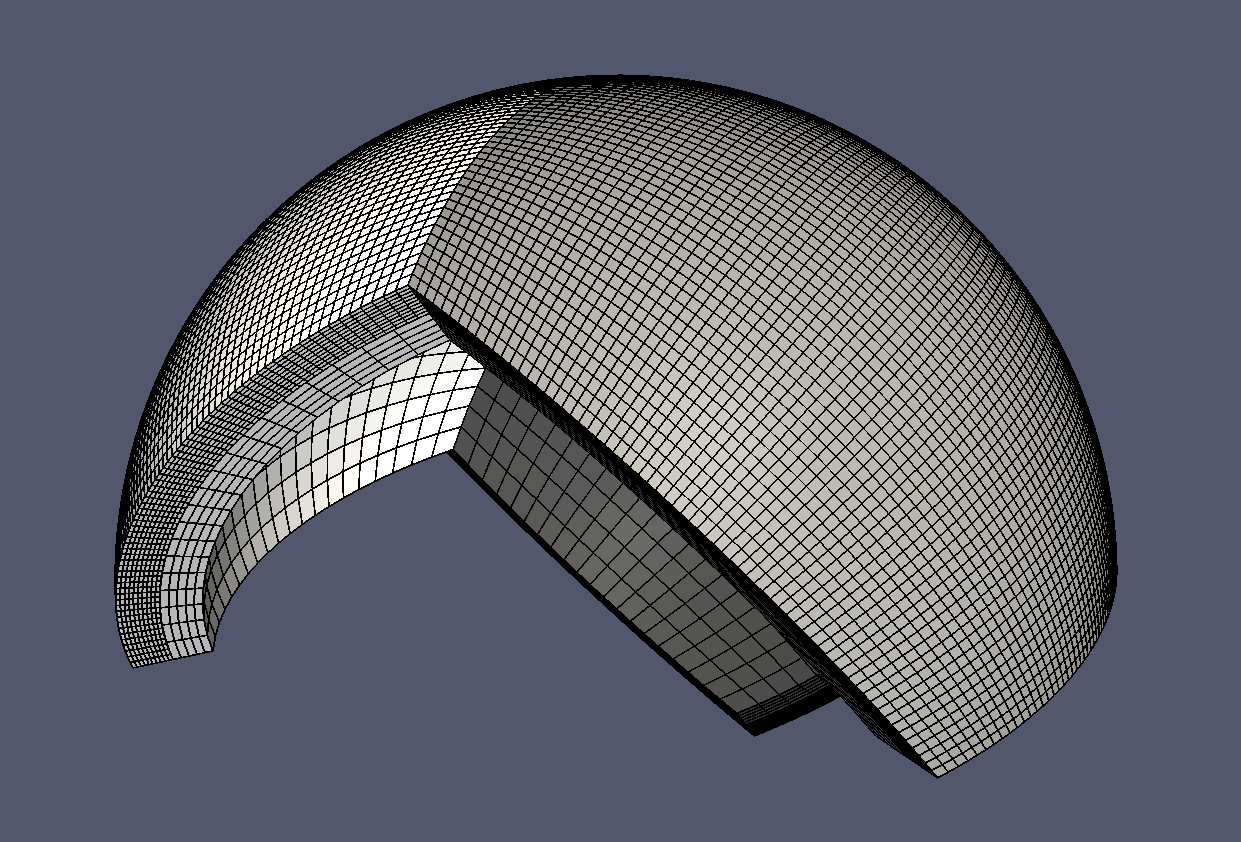
\includegraphics[width=0.65\textwidth]{images/chunksInversionGrid_manual.png}
  \caption{Example of a chunks inversion grid (with 3 chunks in global projection)}
  \label{basic_steps,sec:invgrid,sub:chunks,fig:grid}
\end{figure}

The inversion grid is defined via a paramter file, a template of which is file 
\lcode{template/chunksInversionGrid_parfile_template} (the template file defines the inversion grid
shown in the above figure).
The meaning of the keywords in the parameter file defining an inversion grid of type \lcode{chunksInversionGrid}
are as follows:

\subsubsection{\lcode{CHUNKS_INVGRID_GEOM_NCHUNK}} %\label{files,sec:iter_parfile,itm:invgrid_rad}
Number of chunks (1, 2, 3, or 6).
%- - - - - - - - - - - - - - - - - - - - - - - - - - - - -
\subsubsection{\lcode{CHUNKS_INVGRID_GEOM_RMAX}} 
Maximum radius (upper boundary of the chunk(s)) [must be the same unit in which wavefield points are given, usually be in km]
%- - - - - - - - - - - - - - - - - - - - - - - - - - - - -
\subsubsection{\lcode{CHUNKS_INVGRID_GEOM_CLAT}, \lcode{CHUNKS_INVGRID_GEOM_CLON}} 
Center of cubed-sphere chunk in degrees.
%- - - - - - - - - - - - - - - - - - - - - - - - - - - - -
\subsubsection{\lcode{CHUNKS_INVGRID_GEOM_WLAT}, \lcode{CHUNKS_INVGRID_GEOM_WLON}} 
Assuming \lcode{ROT = 0}.\\
Width of cubed-sphere chunk in degrees (must be 90.0 for NCHUNK $> 1$).
%- - - - - - - - - - - - - - - - - - - - - - - - - - - - -
\subsubsection{\lcode{CHUNKS_INVGRID_GEOM_ROT}} 
Rotation of chunk around local vertical counterclockwise in degrees.
%- - - - - - - - - - - - - - - - - - - - - - - - - - - - -
\subsubsection{\lcode{CHUNKS_INVGRID_BASE_NREF_BLOCKS}}
Number of blocks of layers within which lateral cell width remains comstant.\\
(compare \lcode{scartInversionGrid}~\myref{basic_steps,sec:invgrid,sub:scart}: definition and usage of \lcode{NREF_BLOCKS}, 
\lcode{NLAY}, \lcode{THICKNESS}, \lcode{NX}, \lcode{NY})
%- - - - - - - - - - - - - - - - - - - - - - - - - - - - -
\subsubsection{\lcode{CHUNKS_INVGRID_BASE_NLAY}}
Number of layers within each block (integer array).\\
(compare \lcode{scartInversionGrid}~\myref{basic_steps,sec:invgrid,sub:scart}: definition and usage of \lcode{NREF_BLOCKS}, 
\lcode{NLAY}, \lcode{THICKNESS}, \lcode{NX}, \lcode{NY})
%- - - - - - - - - - - - - - - - - - - - - - - - - - - - -
\subsubsection{\lcode{CHUNKS_INVGRID_BASE_THICKNESS}}
Thickness of layers in each block in km (real array).\\
(compare \lcode{scartInversionGrid}~\myref{basic_steps,sec:invgrid,sub:scart}: definition and usage of \lcode{NREF_BLOCKS}, 
\lcode{NLAY}, \lcode{THICKNESS}, \lcode{NX}, \lcode{NY})
%- - - - - - - - - - - - - - - - - - - - - - - - - - - - -
\subsubsection{\lcode{CHUNKS_INVGRID_BASE_NLAT}, \lcode{CHUNKS_INVGRID_BASE_NLON}}
Number of cells in latitude/longitude direction for each layer block.\\
(compare \lcode{scartInversionGrid}~\myref{basic_steps,sec:invgrid,sub:scart}: definition and usage of \lcode{NREF_BLOCKS}, 
\lcode{NLAY}, \lcode{THICKNESS}, \lcode{NX}, \lcode{NY})
%- - - - - - - - - - - - - - - - - - - - - - - - - - - - -
\subsubsection{\lcode{CHUNKS_INVGRID_FILE}}
Filename of binary inversion grid file (relative to \lcode{MAIN_PATH_INVERSION}/\lcode{ITERATION_STEP_PATH/})
to which a newly created inversion grid will be written and from which the inversion grid
will be read if it exists and if not recreating the inversion grid.
%- - - - - - - - - - - - - - - - - - - - - - - - - - - - -
\subsubsection{\lcode{VTK_PROJECTION}}
\lcode{VTK_PROJECTION} is one of:
\begin{itemize}
\item[]'\lcode{GLOBAL}': center of chunk(s) in \lcode{CLAT}, \lcode{CLON}, with applied \lcode{CHUNKS_INVGRID_GEOM_ROT}
\item[]'\lcode{LOCAL_CURV}': center of chunk in x=y=0, NO \lcode{CHUNKS_INVGRID_GEOM_ROT} applied, but with curvature
\item[]'\lcode{LOCAL_FLAT}': center of chunk in x=y=0, NO \lcode{CHUNKS_INVGRID_GEOM_ROT}, NO curvature, i.e. projection of each depth onto the tangential x-y-plane
\item[]'\lcode{LOCAL_NORTH_CURV}': same as '\lcode{LOCAL_CURV}', but WITH \lcode{CHUNKS_INVGRID_GEOM_ROT} applied, i.e. x really points to south
\item[]'\lcode{LOCAL_NORTH_FLAT}': same as '\lcode{LOCAL_FLAT}', but WITH \lcode{CHUNKS_INVGRID_GEOM_ROT} applied, i.e. x really points to south
\end{itemize}
%- - - - - - - - - - - - - - - - - - - - - - - - - - - - -
\subsubsection{\lcode{VTK_GEOMETRY_TYPE}}
Select the geometry type. \lcode{VTK_GEOMETRY_TYPE} is one of:
\begin{itemize}
\item[]'\lcode{CELLS}': data on inversion grids will be written on the volumetric inversion grid CELLS (hexahedral) to vtk files (as \lcode{UNSTRUCTURED_GRID} datasets) $\rightarrow$ intuitive volumetric view
\item[]'\lcode{CELL_CENTERS}': data on inversion grids will be written on the cell center POINTS to vtk files (as \lcode{POLYDATA} datasets) $\rightarrow$ smaller files, better to apply filters in ParaView
\end{itemize}
%- - - - - - - - - - - - - - - - - - - - - - - - - - - - -
\subsubsection{\lcode{SCALE_VTK_COORDS}, \lcode{VTK_COORDS_SCALING_FACTOR}}
Scale vtk geometry coordinates by factor \lcode{VTK_COORDS_SCALING_FACTOR}, if \lcode{SCALE_VTK_COORDS = .True.}
this may be helpful if coordinate values (e.g. in m) get so large that they cause problems in paraview.
%
%----------------------------------------------------------
\subsection{\lcodetitle{schunkInversionGrid}} \label{basic_steps,sec:invgrid,sub:schunk}
%----------------------------------------------------------
The spherical chunk inversion grid is derived from a simple planar cartesian
grid by projection of each grid plane onto a spherical shell, assuming that
the cartesian grid plane touches the spherical shell at its center.
Since cells have uniform size in the planar cartesian grid plane, cells
on the spherical shell become successively smaller with distance from the 
center of the spherical chunk. Radially, the inversion grid may consist of
several layer blocks each of which may have its own cell size.\\
To describe points in the spherical chunk, we either use LOCAL cartesian coordinates
with the center of the chunk at x=y=0 and z=r, or GLOBAL cartesian coordinates
with z pointing towards the north pole, x pointing towards the equator at lon=0
and y pointing towards the equator at lon=90.\\
The center of the chunk may be shifted to any place on the sphere and, in addition,
may be rotated counterclockwise around its local vertical.

\begin{figure}[ht]
  \centering
  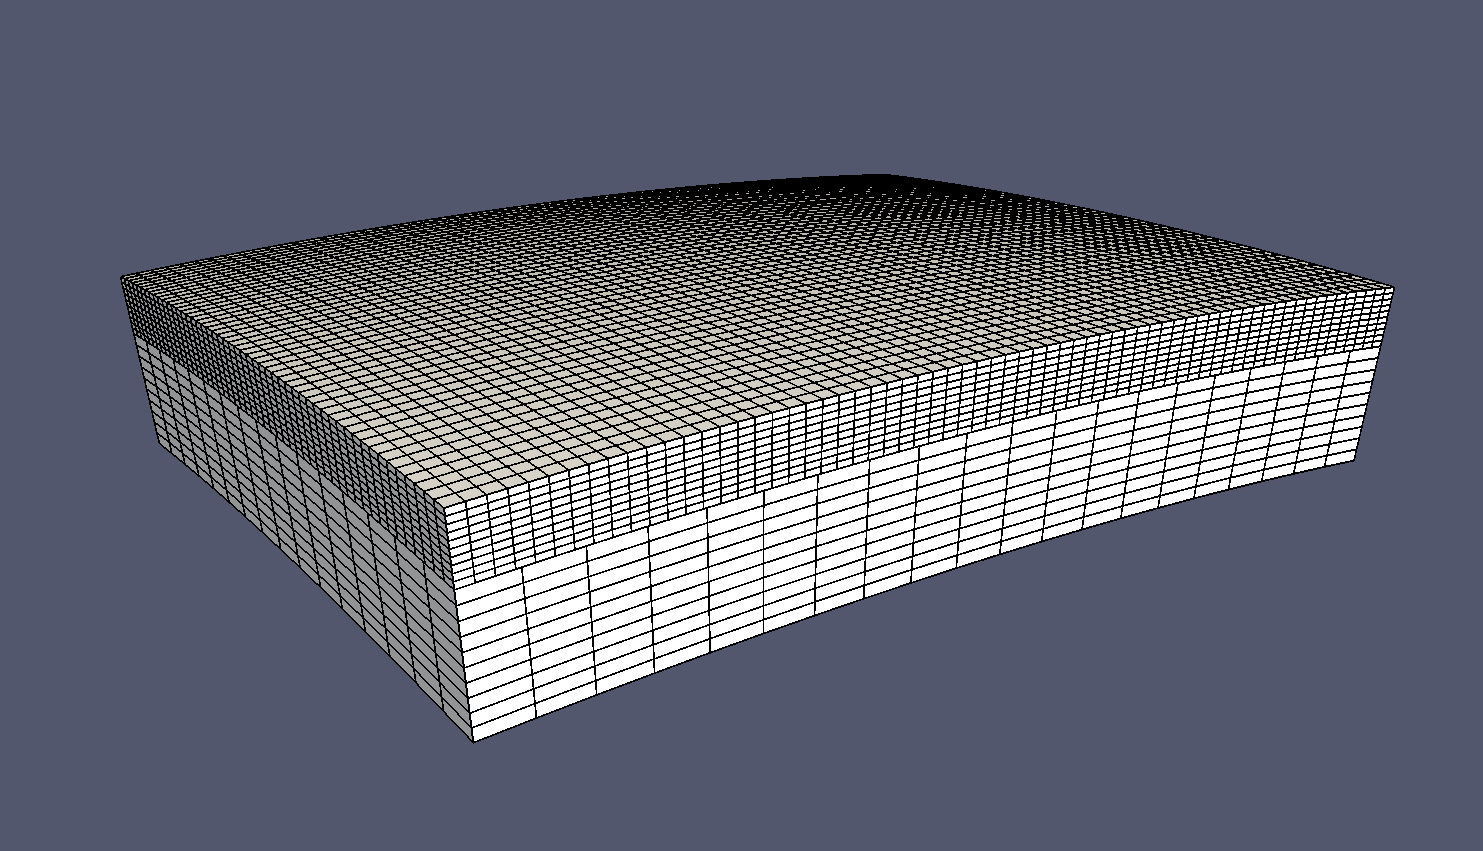
\includegraphics[width=0.65\textwidth]{images/schunkInversionGrid_manual.png}
  \caption{Example of a simple chunk inversion grid (global projection, note the slight curvature of the small chunk)}
  \label{basic_steps,sec:invgrid,sub:schunk,fig:grid}
\end{figure}

The inversion grid is defined via a paramter file, a template of which is file 
\lcode{template/schunkInversionGrid_parfile_template} (the template file defines the inversion grid
shown in the above figure).
The meaning of the keywords in the parameter file defining an inversion grid of type \lcode{schunkInversionGrid}
are as follows:

\subsubsection{\lcode{SCHUNK_INVGRID_CLAT},\lcode{SCHUNK_INVGRID_CLON}} %\label{files,sec:iter_parfile,itm:invgrid_rad} 
Geographic latitude/longitude of center of spherical chunk in degrees.
%- - - - - - - - - - - - - - - - - - - - - - - - - - - - -
\subsubsection{\lcode{SCHUNK_INVGRID_RMAX}}
Maximum radius (upper boundary of spherical chunk) in km.
%- - - - - - - - - - - - - - - - - - - - - - - - - - - - -
\subsubsection{\lcode{SCHUNK_INVGRID_WLAT}, \lcode{SCHUNK_INVGRID_WLON}}
Assuming \lcode{ROT = 0}.\\
Width of spherical chunk parallel to longitude/latitude in degrees.
%- - - - - - - - - - - - - - - - - - - - - - - - - - - - -
\subsubsection{\lcode{SCHUNK_INVGRID_ROT}}
Rotation of chunk around local vertical counterclockwise in degrees.
%- - - - - - - - - - - - - - - - - - - - - - - - - - - - -
\subsubsection{\lcode{SCHUNK_INVGRID_NREF_BLOCKS}}
Number of blocks of layers within which lateral cell width remains constant.\\
(compare \lcode{scartInversionGrid}~\myref{basic_steps,sec:invgrid,sub:scart}: definition and usage of \lcode{NREF_BLOCKS}, 
\lcode{NLAY}, \lcode{THICKNESS}, \lcode{NX}, \lcode{NY})
%- - - - - - - - - - - - - - - - - - - - - - - - - - - - -
\subsubsection{\lcode{SCHUNK_INVGRID_NLAY}}
Number of layers within each block (integer array).\\
(compare \lcode{scartInversionGrid}~\myref{basic_steps,sec:invgrid,sub:scart}: definition and usage of \lcode{NREF_BLOCKS}, 
\lcode{NLAY}, \lcode{THICKNESS}, \lcode{NX}, \lcode{NY})
%- - - - - - - - - - - - - - - - - - - - - - - - - - - - -
\subsubsection{\lcode{SCHUNK_INVGRID_THICKNESS}}
Thickness of layers in each block in km (real array).\\
(compare \lcode{scartInversionGrid}~\myref{basic_steps,sec:invgrid,sub:scart}: definition and usage of \lcode{NREF_BLOCKS}, 
\lcode{NLAY}, \lcode{THICKNESS}, \lcode{NX}, \lcode{NY})
%- - - - - - - - - - - - - - - - - - - - - - - - - - - - -
\subsubsection{\lcode{SCHUNK_INVGRID_NLAT}, \lcode{SCHUNK_INVGRID_NLON}}
Number of cells in latitude/longitude direction for each layer block.\\
(compare \lcode{scartInversionGrid}~\myref{basic_steps,sec:invgrid,sub:scart}: definition and usage of \lcode{NREF_BLOCKS}, 
\lcode{NLAY}, \lcode{THICKNESS}, \lcode{NX}, \lcode{NY})
%- - - - - - - - - - - - - - - - - - - - - - - - - - - - -
\subsubsection{\lcode{VTK_PROJECTION}}
\lcode{VTK_PROJECTION} is one of:
\begin{itemize}
\item[] '\lcode{GLOBAL}': center of chunk in \lcode{CLAT}, \lcode{CLON}, with applied \lcode{SCHUNK_INVGRID_ROT}
\item[] '\lcode{LOCAL_CURV}': center of chunk in x=y=0, NO \lcode{SCHUNK_INVGRID_ROT} applied, but with curvature
\item[] '\lcode{LOCAL_FLAT}': center of chunk in x=y=0, NO \lcode{SCHUNK_INVGRID_ROT} applied, NO curvature, i.e. projection of each depth onto the tangential x-y-plane
\item[] '\lcode{LOCAL_NORTH_CURV}': same as '\lcode{LOCAL_CURV}', but WITH \lcode{SCHUNK_INVGRID_ROT} applied, i.e. x really points to south
\item[] '\lcode{LOCAL_NORTH_FLAT}': same as '\lcode{LOCAL_FLAT}', but WITH \lcode{SCHUNK_INVGRID_ROT} applied, i.e. x really points to south
\end{itemize}
%- - - - - - - - - - - - - - - - - - - - - - - - - - - - -
\subsubsection{\lcode{VTK_GEOMETRY_TYPE}}
Select the geometry type. \lcode{VTK_GEOMETRY_TYPE} is one of:
\begin{itemize}
\item[]'\lcode{CELLS}': data on inversion grids will be written on the volumetric inversion grid CELLS (hexahedral) to vtk files (as \lcode{UNSTRUCTURED_GRID} datasets) $\rightarrow$ intuitive volumetric view
\item[]'\lcode{CELL_CENTERS}': data on inversion grids will be written on the cell center POINTS to vtk files (as \lcode{POLYDATA} datasets) $\rightarrow$ smaller files, better to apply filters in ParaView
\end{itemize}
%- - - - - - - - - - - - - - - - - - - - - - - - - - - - -
\subsubsection{\lcode{SCALE_VTK_COORDS}, \lcode{VTK_COORDS_SCALING_FACTOR}}
Scale all VTK point coordinates by an additional factor,
if \lcode{SCALE_VTK_COORDS = .false.}, then \lcode{VTK_COORDS_SCALING_FACTOR} is ignored.
%- - - - - - - - - - - - - - - - - - - - - - - - - - - - -
%
%----------------------------------------------------------
\subsection{\lcodetitle{scartInversionGrid}} \label{basic_steps,sec:invgrid,sub:scart}
%----------------------------------------------------------
%
A \lcode{S}imple \lcode{CART}esian inversion grid covers a Cartesian cuboid which can
be shifted to a certain location in Cartesian space and may be rotated about the local vertical
axis. Its cells are distributed in layers. Each layer has a certain thickness and a regularly
distributed number of inversion grid cells along each lateral direction of the cuboid.

Please consult the documentation of your forward method (\myref{basic_steps,sec:forward_problem}) if it supports
inversion grids of type \lcode{scartInversionGrid}. \\
All coordinates, e.g.\ of events and stations or wavefield points, are interpreted by this type of inversion grid as
\lcode{X} (first coordinate), \lcode{Y} (second coordinate), \lcode{Z} (third coordinate). Their
units (e.g.\ meters or kilometers) are not assumed by the inversion grid and are essentially defined by the wavefield
points, hence, they might be method dependent and must be overall consistend.\\
Every type of integration weights is supported by this type of inversion grid, except weights of type 
\lcode{6} (external integration weights).

\begin{figure}[ht]
  \centering
  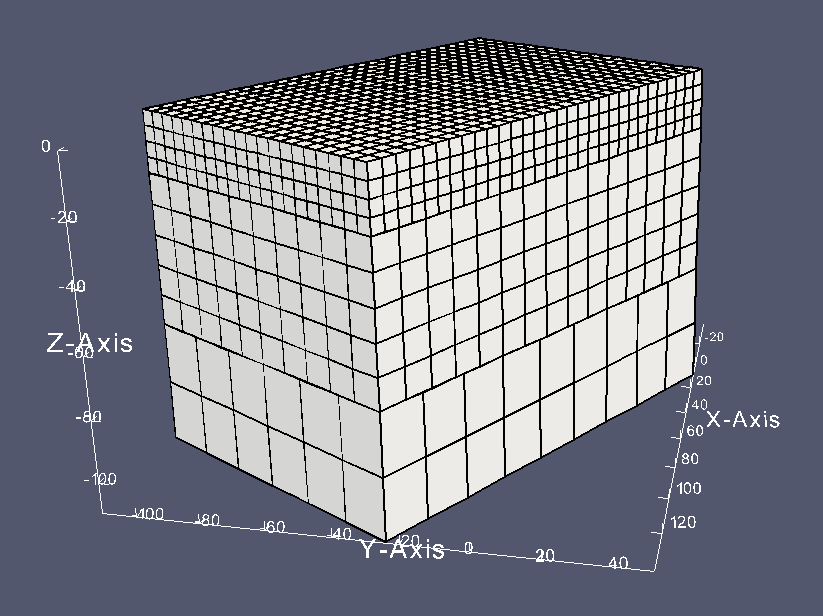
\includegraphics[width=0.5\textwidth]{images/scartInversionGrid_manual.png}
  \caption{Example of a simple Cartesian inversion grid}
  \label{basic_steps,sec:invgrid,sub:scart,fig:grid}
\end{figure}

The shape of the cuboid, as well as the distribution of inversion grid cells, are defined 
via a paramter file, a template of which is file \lcode{template/scartInversionGrid_parfile_template}.
In the following, the particular parameters are explained, with the example
values always refering to the inversion grid as displayed in figure~\myref{basic_steps,sec:invgrid,sub:scart,fig:grid}.

%- - - - - - - - - - - - - - - - - - - - - - - - - - - - - 
\subsubsection{\lcode{SCART_INVGRID_CX}}
\lcode{X}-coordinate of center of cuboid (real number)\\
Example:\\
\lcode{SCART_INVGRID_CX = 50.0}
%- - - - - - - - - - - - - - - - - - - - - - - - - - - - - 
\subsubsection{\lcode{SCART_INVGRID_CY}}
\lcode{Y}-coordinate of center of cuboid (real number)\\
Example:\\
\lcode{SCART_INVGRID_CY = -30.0}
%- - - - - - - - - - - - - - - - - - - - - - - - - - - - - 
\subsubsection{\lcode{SCART_INVGRID_ZMAX}}
Maximum \lcode{Z}-coordinate of cuboid (real number), i.e.\ \lcode{Z}-coordinate of the 
``surface'' of the inversion grid\\
Example:\\
\lcode{SCART_INVGRID_ZMAX = 0.0}
%- - - - - - - - - - - - - - - - - - - - - - - - - - - - - 
\subsubsection{\lcode{SCART_INVGRID_WX}}
Width of cuboid in \lcode{X}-direction (real number)\\
Example:\\
\lcode{SCART_INVGRID_WX = 100.0}
%- - - - - - - - - - - - - - - - - - - - - - - - - - - - - 
\subsubsection{\lcode{SCART_INVGRID_WY}}
Width of cuboid in \lcode{Y}-direction (real number)\\
Example:\\
\lcode{SCART_INVGRID_WY = 150.0}
%- - - - - - - - - - - - - - - - - - - - - - - - - - - - - 
\subsubsection{\lcode{SCART_INVGRID_ROT}}
Angle in degrees of anti-clockwise rotation about the local \lcode{Z}-axis through the 
lateral center of the cuboid (real number)\\
Example:\\
\lcode{SCART_INVGRID_ROT = 60.0}
%- - - - - - - - - - - - - - - - - - - - - - - - - - - - - 
\subsubsection{\lcode{SCART_INVGRID_NREF_BLOCKS,SCART_INVGRID_NLAY,SCART_INVGRID_THICKNESS}}
For an arbitrary number of \lcode{SCART_INVGRID_NREF_BLOCKS} blocks of layers,
the vectors \lcode{SCART_INVGRID_NLAY} (integer values) and \lcode{SCART_INVGRID_THICKNESS} (real values), 
both of length \lcode{SCART_INVGRID_NREF_BLOCKS}, define the \lcode{Z}-direction refinement of each block,
whereby \lcode{SCART_INVGRID_NLAY(i)} defines the number of layers in block \lcode{i}, and 
\lcode{SCART_INVGRID_THICKNESS(i)} defines the thickness of all layers contained in block \lcode{i}.\\
Hence, the overall \lcode{Z}-direction coverage of the inversion grid is defined by 
\lcode{SCART_INVGRID_ZMAX} (which is the coordinate of the top of the first layer in the first refinement block)
and \lcode{SCART_INVGRID_ZMAX - SUM_i(THICKNESS(i) * NLAY(i))} (coordinate of the bottom of the last layer in
%and \lstinline[breaklines=true]$SCART_INVGRID_ZMAX - SUM_i(THICKNESS(i) * NLAY(i))$ (coordinate of the bottom of the last layer in
%and \nolinkurl{SCART_INVGRID_ZMAX - SUM_i(THICKNESS(i) * NLAY(i))} (coordinate of the bottom of the last layer in
last refinement block).\\
Example:\\
\lcode{SCART_INVGRID_NREF_BLOCKS =  3}\\
\lcode{SCART_INVGRID_NLAY =  4   5   2}\\
\lcode{SCART_INVGRID_THICKNESS =  5.0  10.0  20.0}
%- - - - - - - - - - - - - - - - - - - - - - - - - - - - - 
\subsubsection{\lcode{SCART_INVGRID_NX}}
Vector (of length \lcode{SCART_INVGRID_NREF_BLOCKS}) of integer values, defining number of 
inversion grid cells in \lcode{X}-direction, one value for each refinement block\\
Example:\\
\lcode{SCART_INVGRID_NX = 20 10 6}
%- - - - - - - - - - - - - - - - - - - - - - - - - - - - - 
\subsubsection{\lcode{SCART_INVGRID_NY}}
Vector (of length \lcode{SCART_INVGRID_NREF_BLOCKS}) of integer values, defining number of 
inversion grid cells in \lcode{Y}-direction, one value for each refinement block\\
Example:\\
\lcode{SCART_INVGRID_NX = 30 15 9}
%- - - - - - - - - - - - - - - - - - - - - - - - - - - - - 
\subsubsection{\lcode{USE_LOCAL_INVGRID_COORDS_FOR_VTK}}
Logical value to indicate whether to use local inversion grid coordinates for vtk geometry, i.e.\ no rotation 
by \lcode{SCART_INVGRID_ROT} and no shift by \lcode{SCART_INVGRID_CX}, \lcode{SCART_INVGRID_CY}, 
\lcode{SCART_INVGRID_ZMAX} (cuboid centered in \lcode{X=Y=0} and \lcode{ZMAX=0})\\
Example:\\
\lcode{USE_LOCAL_INVGRID_COORDS_FOR_VTK = .false.}
%- - - - - - - - - - - - - - - - - - - - - - - - - - - - -
\subsubsection{\lcode{VTK_GEOMETRY_TYPE}}
Select the geometry type. \lcode{VTK_GEOMETRY_TYPE} is one of:
\begin{itemize}
\item[]'\lcode{CELLS}': data on inversion grids will be written on the volumetric inversion grid CELLS (hexahedral) to vtk files (as \lcode{UNSTRUCTURED_GRID} datasets) $\rightarrow$ intuitive volumetric view
\item[]'\lcode{CELL_CENTERS}': data on inversion grids will be written on the cell center POINTS to vtk files (as \lcode{POLYDATA} datasets) $\rightarrow$ smaller files, better to apply filters in ParaView
\end{itemize}
%- - - - - - - - - - - - - - - - - - - - - - - - - - - - - 
\subsubsection{\lcode{SCALE_VTK_COORDS,VTK_COORDS_SCALING_FACTOR}}
Scale vtk geometry coordinates by factor \lcode{VTK_COORDS_SCALING_FACTOR} (real number), if 
\lcode{SCALE_VTK_COORDS = .true.}. This may be helpful if coordinate values (e.g.\ in meters) 
get so large that they cause problems when plotting in paraview.\\
Example:\\
\lcode{SCALE_VTK_COORDS = .false.}\\
\lcode{VTK_COORDS_SCALING_FACTOR = 1.0}
%- - - - - - - - - - - - - - - - - - - - - - - - - - - - - 
%
%----------------------------------------------------------
\subsection{\lcodetitle{ecartInversionGrid}} \label{basic_steps,sec:invgrid,sub:ecart}
%----------------------------------------------------------
%
{\bf EXPERIMENTAL FEATURE:} \emph{so far, this type of inversion grid works for tetrahedral cells only,
since support for hexahedreal cells is not completed throughout. However, even for tetrahedra the automatic detection 
of neighbours did not work properly in some test cases! So if you intend to use this inversion grid, please have a look 
at the grid and all neighbours (neighbours only required for model smoothing in case of solving the Kernel system of equations).
You can do that by using executable} \lcode{invgrid2vtk} \emph{along with option} \lcode{-nb} \emph{. Execute} 
\lcode{invgrid2vtk} \emph{(without arguments)} \myaref{programs_scripts,sec:bin_prog,sec:invgrid_vtk} \emph{for further details on how to use it.}

An \lcode{E}xternal \lcode{CART}esian inversion grid is defined by several text files containing the definintion 
of nodes (i.e.\  essentially the corner points, or rather the control nodes of the inversion grid cells) and the 
definition of cells by refering to the nodes. At the moment, 4-node tetrahedral cells are fully supported, and 8-node 
hexahedral cells are partly supported. 
Those files may be produced by any meshing tool. In case you are interested to export meshes your own way, 
section~\myref{files,sec:ecart_invgrid} defines the required file formats.\\
\ASKI{} provides the \lcode{python} module \lcode{cubit2ASKIecartInversionGrid.py} which can be used with the 
meshing software \lcode{Cubit} in a \lcode{python} script by first importing the module:\\
\lcode{import cubit2ASKIecartInversionGrid}\\
and at the very end of your meshing process calling:\\
\lcode{cubit.cmd('compress all')}\\
\lcode{cubit2ASKIecartInversionGrid.export2ASKI('EXPORT_PATH')}\\
whereby you may replace \lcode{EXPORT_PATH} by some location where the output files will be written.

Please consult the documentation of your forward method (\myref{basic_steps,sec:forward_problem}) if it supports
inversion grids of type \lcode{ecartInversionGrid}. \\
All coordinates, e.g.\ of events and stations or wavefield points, are interpreted by this type of inversion grid as
\lcode{X} (first coordinate), \lcode{Y} (second coordinate), \lcode{Z} (third coordinate). Their
units (e.g.\ meters or kilometers) are not assumed by the inversion grid and are essentially defined by the wavefield
points, hence, they might be method dependent and must be overall consistend.\\
Every type of integration weights is supported by this type of inversion grid, except weights of type 
\lcode{6} (external integration weights).

\begin{figure}[ht]
  \centering
  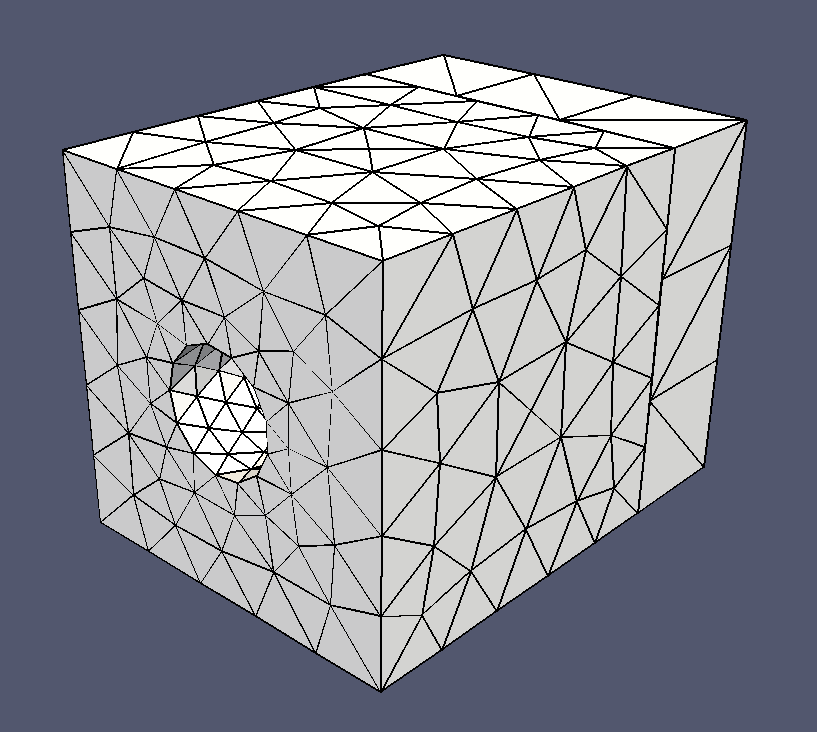
\includegraphics[width=0.5\textwidth]{images/ecartInversionGrid_manual.png}
  \caption{Example of an external Cartesian inversion grid created by Cubit}
  \label{basic_steps,sec:invgrid,sub:ecart,fig:grid}
\end{figure}

The nodes and cell files, e.g.\ produced by \lcode{Cubit}, are referred to in a parameter file, a template 
of which is file \lcode{template/ecartInversionGrid_parfile_template}. In the following, the particular 
parameters are explained. An example inversion grid of this type is displayed in 
figure~\myref{basic_steps,sec:invgrid,sub:ecart,fig:grid}.

%- - - - - - - - - - - - - - - - - - - - - - - - - - - - - 
\subsubsection{\lcode{ECART_INVGRID_USE_NODES_COMMON}}
Logical value to indicate whether to use one common nodes coordinates file for 
all cell types (only use parameter \lcode{ECART_INVGRID_FILE_NODES} below), or to use an individual 
nodes coordinates file for each cell type (use parameters files \lcode{ECART_INVGRID_FILE_NODES_TET4}, 
\lcode{ECART_INVGRID_FILE_NODES_HEX8}, \dots below).\\
When using module \lcode{cubit2ASKIecartInversionGrid} you should set:\\
\lcode{ECART_INVGRID_USE_NODES_COMMON = .True.}
%- - - - - - - - - - - - - - - - - - - - - - - - - - - - - 
\subsubsection{\lcode{ECART_INVGRID_FILE_NODES_COMMON}}
File name relative to \lcode{MAIN_PATH_INVERSION/ITERATION_STEP_PATH/} of nodes coordinates file to be commonly used
for definition of cells of all types in case of \lcode{ECART_INVGRID_USE_NODES_COMMON = .True.}\\
When using module \lcode{cubit2ASKIecartInversionGrid} you should set:\\
\lcode{ECART_INVGRID_FILE_NODES_COMMON = node_coordinates}
%- - - - - - - - - - - - - - - - - - - - - - - - - - - - - 
\subsubsection{\lcode{ECART_INVGRID_FILE_NODES_TET4}}
File name relative to \lcode{MAIN_PATH_INVERSION/ITERATION_STEP_PATH/} of nodes coordinates file to be used
for definition of tet4-type cells in case of \lcode{ECART_INVGRID_USE_NODES_COMMON = .False.}\\
%- - - - - - - - - - - - - - - - - - - - - - - - - - - - - 
\subsubsection{\lcode{ECART_INVGRID_FILE_NODES_HEX8}}
File name relative to \lcode{MAIN_PATH_INVERSION/ITERATION_STEP_PATH/} of nodes coordinates file to be used
for definition of hex8-type cells in case of \lcode{ECART_INVGRID_USE_NODES_COMMON = .False.}\\
%- - - - - - - - - - - - - - - - - - - - - - - - - - - - - 
\subsubsection{\lcode{ECART_INVGRID_FILE_CELLS_TET4}}
File name relative to \lcode{MAIN_PATH_INVERSION/ITERATION_STEP_PATH/} of cell connectivity file for 
definition of tet4-type cells.\\
When using module \lcode{cubit2ASKIecartInversionGrid} you should set:\\
\lcode{ECART_INVGRID_FILE_CELLS_TET4 = cell_connectivity_tet4}
%- - - - - - - - - - - - - - - - - - - - - - - - - - - - - 
\subsubsection{\lcode{ECART_INVGRID_FILE_CELLS_HEX8}}
File name relative to \lcode{MAIN_PATH_INVERSION/ITERATION_STEP_PATH/} of cell connectivity file for 
definition of hex8-type cells.\\
When using module \lcode{cubit2ASKIecartInversionGrid} you should set:\\
\lcode{ECART_INVGRID_FILE_CELLS_HEX8 = cell_connectivity_hex8}
%- - - - - - - - - - - - - - - - - - - - - - - - - - - - - 
\subsubsection{\lcode{ECART_INVGRID_FILE_NEIGHBOURS}}
File name relative to \lcode{MAIN_PATH_INVERSION/ITERATION_STEP_PATH/} of cell neighbours file. If not
present, this file will be created when first using the inversion grid. If present, its content defines 
the neighbour structure of the inversion grid cells. If, however, the inversion grid
is to be recreated (e.g.\ when calling \lcode{initBasics -recr}, see section~\myref{basic_steps,sec:initBasics}),
this file is recreated.
%- - - - - - - - - - - - - - - - - - - - - - - - - - - - - 
\subsubsection{\lcode{ECART_INVGRID_FILE_NEIGHBOURS_IS_BINARY}}
Logical value to indicate whether \lcode{ECART_INVGRID_FILE_NEIGHBOURS} should be binary or not.
%- - - - - - - - - - - - - - - - - - - - - - - - - - - - -
\subsubsection{\lcode{VTK_GEOMETRY_TYPE}}
Select the geometry type. \lcode{VTK_GEOMETRY_TYPE} is one of:
\begin{itemize}
\item[]'\lcode{CELLS}': data on inversion grids will be written on the volumetric inversion grid CELLS (hexahedral) to vtk files (as \lcode{UNSTRUCTURED_GRID} datasets) $\rightarrow$ intuitive volumetric view
\item[]'\lcode{CELL_CENTERS}': data on inversion grids will be written on the cell center POINTS to vtk files (as \lcode{POLYDATA} datasets) $\rightarrow$ smaller files, better to apply filters in ParaView
\end{itemize}
%- - - - - - - - - - - - - - - - - - - - - - - - - - - - - 
\subsubsection{\lcode{SCALE_VTK_COORDS,VTK_COORDS_SCALING_FACTOR}}
Scale vtk geometry coordinates by factor \lcode{VTK_COORDS_SCALING_FACTOR} (real number), if 
\lcode{SCALE_VTK_COORDS = .true.}. This may be helpful if coordinate values (e.g.\ in meters) 
get so large that they cause problems when plotting in paraview.\\
Example:\\
\lcode{SCALE_VTK_COORDS = .false.}\\
\lcode{VTK_COORDS_SCALING_FACTOR = 1.0}
%
%----------------------------------------------------------
\subsection{\lcodetitle{specfem3dInversionGrid}} \label{basic_steps,sec:invgrid,sub:specfem3d}
%----------------------------------------------------------
%
An inversion grid of type \lcode{specfem3dInversionGrid} is method dependent and is to be used with 
\lcode{METHOD = SPECFEM3D} only. Whole spectral elements are used as inversion grid cells and all 
GLL points inside such an element as the wavefield points. All information regarding the element 
geometry, including information on neighbour cells and the values of the jacobian for every wavefield 
point contained in an element are read from files which are produced by \lcode{SPECFEM3D} methods.

Every type of integration weights is supported by this type of inversion grid, including weights of type 
\lcode{6} (external integration weights, i.e.\ the very integration weights that already \lcode{SPECFEM3D}
uses to integrate over spectral elements).

Please refer to the documentation of your \lcode{SPECFEM3D} forward method (\myref{basic_steps,sec:forward_problem})
on how to generate any files required for using an inversion grid of type \lcode{specfem3dInversionGrid}.

As with all other types of inversion grids, a parameter file defines any details of the grid, a template 
of which is file \lcode{template/specfem3dInversionGrid_parfile_template}.
In the following, the particular parameters are explained.

%- - - - - - - - - - - - - - - - - - - - - - - - - - - - - 
\subsubsection{\lcode{SPECFEM3D_ASKI_MAIN_FILE}}
File name relative to \lcode{MAIN_PATH_INVERSION/ITERATION_STEP_PATH/} of file from \lcode{SPECFEM3D}
containing all information about the inversion grid (any \lcode{.main} output file)\\
Example:\\
\lcode{SPECFEM3D_ASKI_MAIN_FILE = kernel_displacements/kernel_displ_S001.main}
%- - - - - - - - - - - - - - - - - - - - - - - - - - - - -
\subsubsection{\lcode{VTK_GEOMETRY_TYPE}}
Select the geometry type. \lcode{VTK_GEOMETRY_TYPE} is one of:
\begin{itemize}
\item[]'\lcode{CELLS}': data on inversion grids will be written on the volumetric inversion grid CELLS (hexahedral) to vtk files (as \lcode{UNSTRUCTURED_GRID} datasets) $\rightarrow$ intuitive volumetric view
\item[]'\lcode{CELL_CENTERS}': data on inversion grids will be written on the cell center POINTS to vtk files (as \lcode{POLYDATA} datasets) $\rightarrow$ smaller files, better to apply filters in ParaView
\end{itemize}
%- - - - - - - - - - - - - - - - - - - - - - - - - - - - - 
\subsubsection{\lcode{SCALE_VTK_COORDS,VTK_COORDS_SCALING_FACTOR}}
Scale vtk geometry coordinates by factor \lcode{VTK_COORDS_SCALING_FACTOR} (real number), if 
\lcode{SCALE_VTK_COORDS = .true.}. This may be helpful if coordinate values (e.g.\ in meters) 
get so large that they cause problems when plotting in paraview.\\
Example:\\
\lcode{SCALE_VTK_COORDS = .false.}\\
\lcode{VTK_COORDS_SCALING_FACTOR = 1.0}
%- - - - - - - - - - - - - - - - - - - - - - - - - - - - - 
\subsubsection{\lcode{SPECFEM3D_R_EARTH_KM}}
In case of using \lcode{SPECFEM3D_GLOBE}, define here the maximum radius [km] of the sphere, by which 
Earth is approximated (only used to interpret ``depth'' and ``altitude'' of events and stations when 
plotting to vtk files; ignored for \lcode{SPECFEM3D_Cartesian} applications).\\
Example:\\
\lcode{SPECFEM3D_R_EARTH_KM = 6371.0}
%
%++++++++++++++++++++++++++++++++++++++++++++++++++++++++++
\section{Define a Starting Model} \label{basic_steps,sec:start_model}
%++++++++++++++++++++++++++++++++++++++++++++++++++++++++++
%
There are two possibilities to define an earth model for the forward wave propagation in your first iteration:

On the one hand you may use any (standard) earth model provided by the forward method you are using, if appropriate.

If this is not possible, or the models provided do not meet your needs, you may use executable 
\lcode{createStartmodelKim} along with the inversion grid of your first iteration (which you should 
have already defined) to produce an inverted model file containing some simple model on this inversion grid. 
Executing \lcode{createStartmodelKim} (without arguments) will print a short help message how to use the program 
\myaref{programs_scripts,sec:bin_prog,sec:create_startmod_kim}. Afterwards you may 
export the produced model file to your forward method as explained in section~\myref{basic_steps,sec:export_kim}.
Template files of starting model descriptions may be found in \lcode{template/}.
%
%++++++++++++++++++++++++++++++++++++++++++++++++++++++++++
\section{Export Inverted Model} \label{basic_steps,sec:export_kim}
%++++++++++++++++++++++++++++++++++++++++++++++++++++++++++
%
The executable \lcode{exportKim} exports an inverted model file (``kim'' stands for ``K''ernel 
``I''nverted ``M''odel) along with the respective inversion grid specifications to a text file, 
which may be used to communicate such a model to a forward method or postprocess the model values in any way. 
Executing \lcode{exportKim} (without argument) will print a short help message how to use it 
\myaref{programs_scripts,sec:bin_prog,sec:exp_Kim}.
%
%++++++++++++++++++++++++++++++++++++++++++++++++++++++++++
\section{Solving the Forward Problem} \label{basic_steps,sec:forward_problem}
%++++++++++++++++++++++++++++++++++++++++++++++++++++++++++
%
In the following, all wave propagation codes which are supported by \ASKI{} are listed.
Refer to the given documentation on any details regarding the interaction of the forward codes with \ASKI{}.
\subsection*{\lcode{Gemini II}}
\lcode{Gemini II} (by \cite{friederich_wd1995}) is supported in this release version, for Cartesian as well as spherical setting. 
The \lcode{Gemini} routines producing spectral output for \ASKI{}, however, might not yet be available. 
We hope to be able to provide them in due time. Until now, please contact us via \url{http://www.rub.de/aski}
if you want to use \lcode{Gemini II} as a forward solver for \ASKI{}.
\subsection*{\lcode{SPECFEM3D_Cartesian}}
The Cartesian spectral element code \lcode{SPECFEM3D_Cartesian} (by \cite{TrKoLi08}), 
version \lcode{3.0} is fully supported by this \ASKI{} release version, cf.~\cite{Specfem3D_Cartesian_for_ASKI}.
\subsection*{\lcode{SPECFEM3D_GLOBE}}
The global spectral element code \lcode{SPECFEM3D_GLOBE} (by \cite{TrKoLi08}), 
version \lcode{7.0.0}, is fully supported by this \ASKI{} release version, cf.~\cite{Specfem3D_Globe_for_ASKI}.
\subsection*{\lcode{NEXD}}
The nodal discontinous Galerkin code \lcode{NEXD} (by \cite{Lambrecht.2015}) is fully supported by this 
\ASKI{} release version. \lcode{NEXD}, including \ASKI{} support, will be available 
under terms of the GPL in the near future via \url{http://www.rub.de/nexd}.
%
%++++++++++++++++++++++++++++++++++++++++++++++++++++++++++
\section{Choose Integration Weights} \label{basic_steps,sec:intw}
%++++++++++++++++++++++++++++++++++++++++++++++++++++++++++
%
In order to numerically integrate the sensitivity kernels, which are computed on the wavefield points, 
over the inversion grid cells by a weightet summation of values, there are different 
types of integration weights provided, following different rules of integration.

The integer values of the type have the following meaning:
\begin{itemize}
  \item[] \lcode{0} $\rightarrow$ all weights are the same, \lcode{weight = 1/number_of_points_in_box}, 
    i.e.\ no integration(!), just building the average sensitivity value (e.g.\ convenient for comparison of 
    sensitivities computed with different methods on different forward grids)
  \item[] \lcode{1} $\rightarrow$ Scattered Data Integration, as in \cite{Levin99}, polynomial degree 1
  \item[] \lcode{2} $\rightarrow$ Scattered Data Integration, as in \cite{Levin99}, polynomial degree 2, 
    i.e.\ approximation order 3 (?)
  \item[] \lcode{3} $\rightarrow$ Scattered Data Integration, as in \cite{Levin99}, polynomial degree 3, 
    i.e.\ approximation order 4 (?)
  \item[] \lcode{4} $\rightarrow$ for each cell, compute the highest possible order of Scattered Data Iintegration
    integration after \cite{Levin99} (trying types 3,2,1 (in that order) until computation was successful)
  \item[] \lcode{5} $\rightarrow$ average of function values, multiplied with volume of box (i.e.\ $\sim$ linear integration)
  \item[] \lcode{6} $\rightarrow$ external integration weights, to be used along with a suitable inversion grid 
    (e.g.\ of type \lcode{specfem3dInversionGrid}, see section~\myref{basic_steps,sec:invgrid,sub:specfem3d})
\end{itemize}

A detailed description of some of the integration weights, especially the weights after \cite{Levin99} can be found in 
section~\myref{programs_scripts,sec:fmod_intw}.
%
%++++++++++++++++++++++++++++++++++++++++++++++++++++++++++
\section{Create a Data and Model Space} \label{basic_steps,sec:dmspace}
%++++++++++++++++++++++++++++++++++++++++++++++++++++++++++
%
In order to choose a set of data samples which to invert and a set of model values which to invert for, 
you need to define a data space and a model space. Essentially, if you have $m$ data samples, the space in which 
the data live is just \R m (analogously, for $n$ model values, the model lives in \R n ). You only need to define which
data sample (model value) refers to which dimension (i.e.\ entry in vector) of the data space (model space), respectively.\\
The $m\times n$ sensitivity kernel matrix will then connect a vector of model updates from model space in \R n 
to your specific data vector from \R m.

In the following, it is described how data samples and model values are characterized in this software package and 
how you can choose specific subsets to be used. 
%----------------------------------------------------------
\subsection{How Data Samples are Characterized}
%----------------------------------------------------------
As the sensitivities are calculated in frequency domain, the data live in frequency domain, too.\\
A data sample is uniquely characterized by a seismic \emph{source}, a \emph{component} 
of a seismic \emph{station}, and a \emph{frequency}, as well as whether it is the \emph{real} or \emph{imaginary} part 
of the complex spectral values. Refer to \myref{basic_steps,sec:data_general} for details on data in \ASKI{}.
%----------------------------------------------------------
\subsection{How Model Values are Characterized} \label{basic_steps,sec:dmspace,sub:mparam}
%----------------------------------------------------------
A model value is uniquely  characterized by a parameter name (must be a valid parameter name of the model
parametrization as defined by \lcode{MODEL_PARAMETRIZATION} \myref{files,sec:main_parfile,itm:mod_pmtrz}) 
and an inversion grid cell index in valid range.
%----------------------------------------------------------
\subsection{How to Define Data and Model Space: Choosing a Set of Data Samples and Model Values}
%----------------------------------------------------------
Create a text file as described in section \myref{files,sec:dmspace}, e.g.\ by adjusting the provided
template files in \lcode{template/}.
%
%++++++++++++++++++++++++++++++++++++++++++++++++++++++++++
\section{Initiate Basic Requirements} \label{basic_steps,sec:initBasics}
%++++++++++++++++++++++++++++++++++++++++++++++++++++++++++
%
Use the executable \lcode{initBasics}. Executing \lcode{initBasics} (without arguments) 
will print a short help message how to use it \myaref{programs_scripts,sec:bin_prog,sec:in_basics}.

It first checks if all parameters needed are present in the parameter files and then creates all
basic requirements for \ASKI{} operations:\\
It reads in required files like event list and station list files, the wavefield points and the 
kernel reference model. \\
Furthermore, it creates the inversion grid (possibly storing some inversion grid files, dependent 
on the type of grid), localizes the wavefield points inside it and computes 
the integration weights, which are written to file. Once those files exist, \lcode{initBasics} 
and all other programs will always read the integration weights (and possibly (part of) the inversion grid) 
from file, \emph{regardless} of what the parameter files say! So if at some you point want to use 
different integration weights or a different inversion grid, you will have to either delete the respective 
file(s) and rerun \lcode{initBasics}, or run \lcode{initBasics -recr} in order
to recreate them. 

Also a lot of \lcode{.vtk} files with statistics are produced having base filename \lcode{FILEBASE_BASIC_STATS} as 
defined in the parameter file of the current iteration step. Those files mainly regard the inversion grid, 
the wavefield points and the integration weights, where the respective filenames are extended (by something 
with ``.vtk''). It is \emph{highly recommended} to call \lcode{initBasics -recr} in order to assure that all
those \lcode{.vtk} files are produced and to actually have a look at them before continuing any \ASKI{} operation!
%
%++++++++++++++++++++++++++++++++++++++++++++++++++++++++++
\section{Compute Spectral Waveform Sensitivity Kernels} \label{basic_steps,sec:compute_kernels}
%++++++++++++++++++++++++++++++++++++++++++++++++++++++++++
%
The kernels are computed by combining green tensor component(s) and forward wavefield for a given event-station
pair (called ``path'' below. By default, the kernels are integrated over the inverison grid cells. I.e.\ there is one sensitivity 
kernel file for a specific event-station path. This file contains sensitivity values of the requested 
station components for the requested model parameters of your model parametrization, with 
the values living on the inverison grid cells. Alternatively, kernels can be computed on the wavefield points,
without pre-integration (for inspection only, cannot be used for waveform inversion in that case).

Use executable \lcode{computeKernels}. Executing \lcode{computeKernels} (without arguments) 
will print a short help message how to use it \myaref{programs_scripts,sec:bin_prog,sec:com_kernel}.
It makes sense, to only compute kernel files for those event-station paths that you are going to use (defined by
your data-model-space file).

You can define the set of event-station paths, station components and model parameters for which 
sensitivities should be computed in two ways:
\begin{itemize}
\item[way 1] compute a kernel for only one event-station path, defined by eventID and station name using options 
\lcode{-evid}, \lcode{-stname}, \lcode{-comp}, \lcode{-param}
\item[way 2] input a data-model-space file (as defined by \myref{basic_steps,sec:dmspace}) by option 
\lcode{-dmspace}, defining all event-station paths and respective station components and model parameters 
for which kernels should be computed; optionally define range of path index
by \lcode{-ipath1}, \lcode{-ipath2}
\end{itemize}
Setting option \lcode{-wp} will compute plain kernel values on wavefield points (no pre-integration onto inversion
grid). \emph{This option will produce separate files, so you can compute both, kernels on wavefield points and
on inversion grid}.
%
%++++++++++++++++++++++++++++++++++++++++++++++++++++++++++
\section{Transform to Time-Domain Sensitivity Kernels} \label{basic_steps,sec:compute_time_kernels}
%++++++++++++++++++++++++++++++++++++++++++++++++++++++++++
%
The time kernels are computed from the standard frequency-domain kernels (which were computed path-wise)
by applying an inverse Fourier transform. 

Use executable \lcode{spec2timeKernels}. Executing \lcode{spec2timeKernels} (without arguments) will print a short
help message how to use it \myaref{programs_scripts,sec:bin_prog,sec:spec_time_kernels}.

The set of event-station paths, station components and model parameters for which time kernels should be produced
are defined in the same ``two ways'' (by the same options) as computing spectral waveform kernels 
\myaref{basic_steps,sec:compute_kernels}.

Additionally, you need to define the time discretization of the produced time kernel by options 
\lcode{-dt}, \lcode{-nt1}, \lcode{-nt2}, \lcode{-t0}.
%
%++++++++++++++++++++++++++++++++++++++++++++++++++++++++++
\section{Plot Spectral Waveform Sensitivity Kernels} \label{basic_steps,sec:plot_kernels}
%++++++++++++++++++++++++++++++++++++++++++++++++++++++++++
%
One way to plot a specific sensitivity Kernel in frequency domain, i.e.\ the sensitivity spectra for a specific
event-station path, is to procuce vtk files using executable \lcode{kernel2vtk}. 
Executing \lcode{kernel2vtk} will print a short help message how to use it \myaref{programs_scripts,sec:bin_prog,sec:kernel_2_vtk}.

Please note, that the output \lcode{.vtk} files (one for every frequency) might get large, dependent on the resolution 
of the inversion grid, since the geometry information of the inversion grid cells is contained in each \lcode{.vtk} file.
If the files become too large for you, you might consider setting \lcode{DEFAULT_VTK_FILE_FORMAT = BINARY} in your 
main parameter file.
%
%++++++++++++++++++++++++++++++++++++++++++++++++++++++++++
\section{Plot Time Sensitivity Kernels} \label{basic_steps,sec:plot_time_kernels}
%++++++++++++++++++++++++++++++++++++++++++++++++++++++++++
%
One way to plot a specific sensitivity Kernel in time domain, is to procuce vtk files using executable \lcode{timeKernel2vtk}. 
Executing \lcode{timeKernel2vtk} (without arguments) will print a short help message how to use it \myaref{programs_scripts,sec:bin_prog,sec:timeKernel_2_vtk}.\\

Please note, that the output \lcode{.vtk} files (one for every time step) might get large, dependent on the resolution 
of the inversion grid, since the geometry information of the inversion grid cells is contained in each \lcode{.vtk} file.
If the files become too large for you, you might consider setting \lcode{DEFAULT_VTK_FILE_FORMAT = BINARY} in your 
main parameter file.
For a lot of time steps, the \lcode{.vtk} file format is actually not optimally chosen by \ASKI{}, since the complete geometry
information is contained in every time-step file (a lot of redundant information is written to hard disc).
%
%++++++++++++++++++++++++++++++++++++++++++++++++++++++++++
\section{Solve Kernel System} \label{basic_steps,sec:solve_kernel_system}
%++++++++++++++++++++++++++++++++++++++++++++++++++++++++++
%
At the moment, there are 3 executable programs implemented which solve the kernel linear system.
\begin{itemize}
\item
\lcode{solveKernelSystem} is a serial program which sets up the kernel matrix, 
reads in synthetic and measured data, adds regularization condutions to the system if 
requested (smoothing, damping) and solves the system based on \lcode{LAPACK} libraries.\\
Executing \lcode{solveKernelSystem} (without arguments) will print a short help message how to use it 
\myaref{programs_scripts,sec:bin_prog,sec:sol_Ker_Sys}.
\item 
\lcode{solveParKernelSystem} does essentially the same as \lcode{solveKernelSystem}, but uses
parallelized \lcode{ScaLAPACK} libraries to solve the (regularized) kernel linear system. You
must compile executable \lcode{solveParKernelSystem} separately (\lcode{make all} does not
compile it, make sure you have \lcode{ScaLAPACK} libraries installed and linked in the 
\lcode{Makefile}).
Executing \lcode{solveParKernelSystem} (without arguments) will print a short help message how to use it 
\myaref{programs_scripts,sec:bin_prog,sec:solve_par_kernel_sys}.
This executable requires an additional parameter file, see template file\\
\lcode{templated/solveParKernelSystem_parfile_template}.
\item 
\lcode{solveCglsrKernelSystem} sets up the (regularized) kernel linear system, as the above
excecutables do, but the uses a conjugate gradient algorithm to solve the kernel linear system
in a least-squares sense \myaref{programs_scripts,sec:bin_prog,sec:solve_cgls_kernel_sys}.
This executable requires an additional parameter file, see template file\\
\lcode{templated/solveCglsKernelSystem_parfile_template}.\\
Executing \lcode{solveCglsKernelSystem} (without arguments) will print a short help message how to use it 
\myaref{programs_scripts,sec:bin_prog,sec:solve_cgls_kernel_sys}.
\end{itemize}
%
%++++++++++++++++++++++++++++++++++++++++++++++++++++++++++
\section{Investigate State of Convergence of Waveform Inversion} \label{basic_steps,sec:investigate_convergence}
%++++++++++++++++++++++++++++++++++++++++++++++++++++++++++
%
These kinds of operations probalby still need further development in \ASKI{}. 

Whenever solving the linear system of kernel equations in an interation step of full waveform inversion
(see above section~\myref{basic_steps,sec:solve_kernel_system}), the current linear misfit is
printed to output files or on screen, i.e.\ the
the sum of residual squares of the linear system of equations. Also the current misfit between synthetics 
and measured data can be computed by executable \lcode{computeMisfit}
\myaref{programs_scripts,sec:bin_prog,sec:comp_misfit}.
However, comparing these two during variation of the regularization parameters does not give sensible
information on which regularization to choose. The development of the non-linear misfit, i.e.\ comparing
synthetic data based on the new models with the measured data, can only be observed after solving the
forward problem for each of the models to choose from. There is not yet an automated way implemented in
\ASKI{} that does this. Evaluating the non-linear misfit, i.e.\ conducting suitable forward calculations, 
would have to be done by hand for the selected models resulting from the selected regularization parameters.

If you would like to do traditional resolution tests, 
executable \lcode{computeDataFromKernelSystem} \myaref{programs_scripts,sec:bin_prog,sec:comp_data_kernel_sys}
computes the ``measured'' data $d$ in the equation $d-s = K (m1 - mref)$ for any given model m1.
This can be used for traditional linear computation of checkerboard data by forward multiplication 
of the sensitivity matrix with an artificial model vector containing checker anomalies.
A model containing checker or spike-like anomalies can be produced by the preliminary hard-coded executable
\lcode{addSpikeCheckerToKim} \myaref{programs_scripts,sec:bin_prog,sec:addSpikeCheckerToKim}.
%
%++++++++++++++++++++++++++++++++++++++++++++++++++++++++++
\section{Path-Specific Approach to an Iteration of Waveform Inversion} \label{basic_steps,sec:path_specific}
%++++++++++++++++++++++++++++++++++++++++++++++++++++++++++
%
\ASKI{} supports a ``path-specific'' approach to an iteration of full waveform inversion, which is enabled
by flag \lcode{USE_PATH_SPECIFIC_MODELS} in the iteration step parameter file \myaref{files,sec:iter_parfile}.

This approach was applied by \cite{Lamara.2015b} in his first iteration of full waveform inversion
using the 1D code Gemini as a forward solver. Due to the complex structure of the investigated region
(Aegean), it was infeasible to choose a single 1D background model for solving the total forward problem. 
Therefore, an individual 1D background model was chosen for each event-station path which explained
the particular seismogram of that path very well. 

This path-specific concept requires to account for different kernel reference models and to introduce a
correction term in the linear system of kernel equations in order to invert for a global 3D model. Any 
required functionality is implemented in \ASKI{} and was successfully applied. We refer to \cite{Lamara.2015b}
and \cite{Schumacher16} on a more detailed description of the concept.

The required quantity of the correction term, called synthetic correction, can be computed in \ASKI{} by 
executable \lcode{computeCorrectionSyntheticData} \myaref{programs_scripts,sec:bin_prog,sec:comp_correct_syn_data}.
